Chương này trình bày kết quả phân tích và so sánh hiệu suất của các thuật toán tổng hợp trọng số trong Federated Learning dựa trên các kết quả thực nghiệm từ các công bố khoa học. Các thuật toán được đánh giá bao gồm FedAvg (baseline), FedLWS, FedAWA, FedNolowe và FedProto.

\section{Thiết lập thực nghiệm}

\subsection{Bộ dữ liệu và phân chia}

Các thí nghiệm được thực hiện trên hai bộ dữ liệu chuẩn:

\begin{table}[!htb]
    \centering
    \caption{Thông tin chi tiết về bộ dữ liệu}
    \label{tab:datasets}
    \renewcommand{\arraystretch}{1.3}
    \begin{tabular}{|l|c|c|c|c|}
        \hline
        \textbf{Dataset} & \textbf{Train} & \textbf{Test} & \textbf{Classes} & \textbf{Image Size} \\
        \hline
        MNIST & 60,000 & 10,000 & 10 & $28 \times 28 \times 1$ \\
        \hline
        CIFAR-10 & 50,000 & 10,000 & 10 & $32 \times 32 \times 3$ \\
        \hline
    \end{tabular}
\end{table}

Dữ liệu được phân chia cho 100 clients theo phân phối Dirichlet với 2 mức độ: Non-IID mạnh ($\alpha = 0.1$) và IID ($\alpha = 100$).

% --- Hình 1 ---
\begin{figure}[H] 
    \centering
    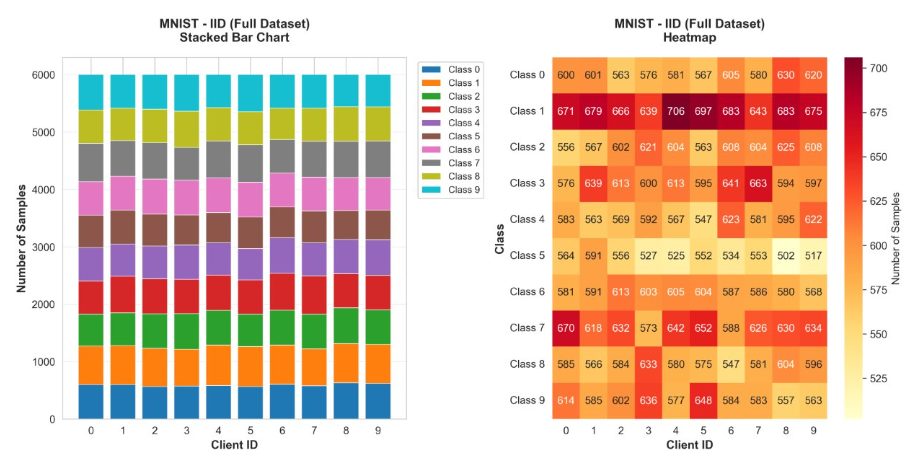
\includegraphics[width=\textwidth]{img/mnist_iid_distribution.png}
    \caption{Phân bố IID trên MNIST}
    \label{fig:mnist_iid}
\end{figure}

% --- Hình 2 ---
\begin{figure}[H]
    \centering
    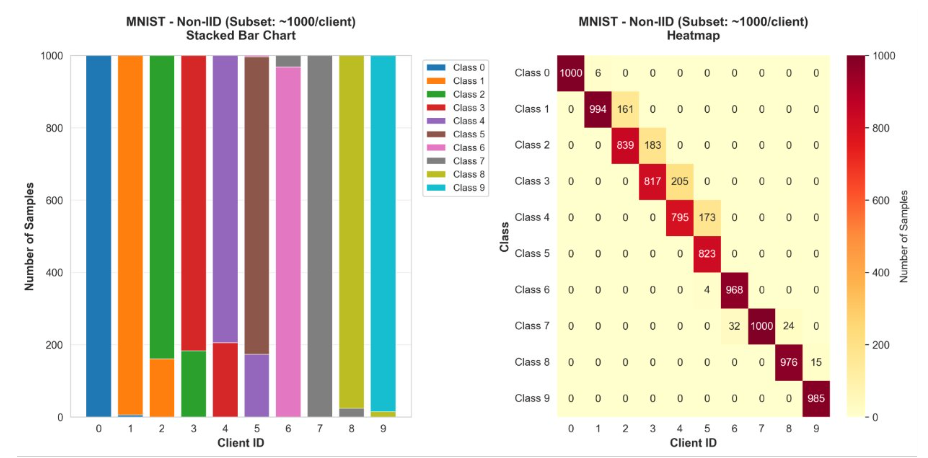
\includegraphics[width=\textwidth]{img/mnist_noniid_distribution.png}
    \caption{Phân bố Non-IID trên MNIST ($\alpha=0.1$)}
    \label{fig:mnist_noniid}
\end{figure}

% --- Hình 3 ---
\begin{figure}[H]
    \centering
    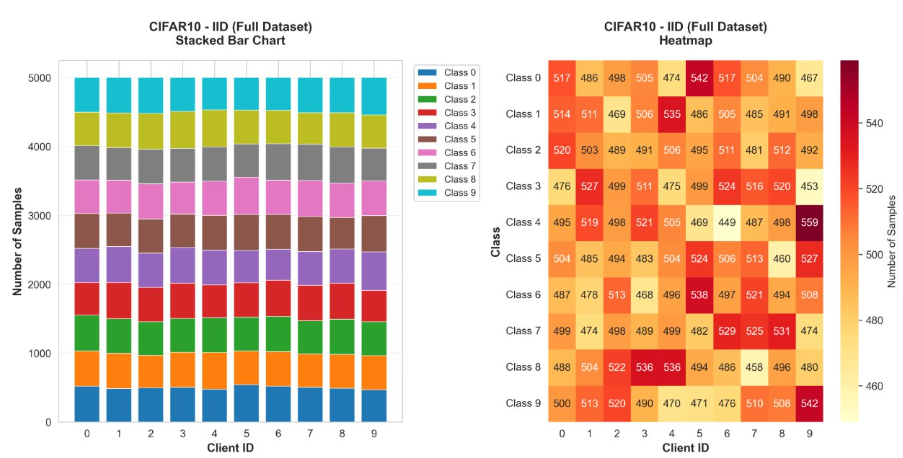
\includegraphics[width=\textwidth]{img/cifar10_iid_distribution.png}
    \caption{Phân bố IID trên CIFAR-10}
    \label{fig:cifar10_iid}
\end{figure}

% --- Hình 4 ---
\begin{figure}[H]
    \centering
    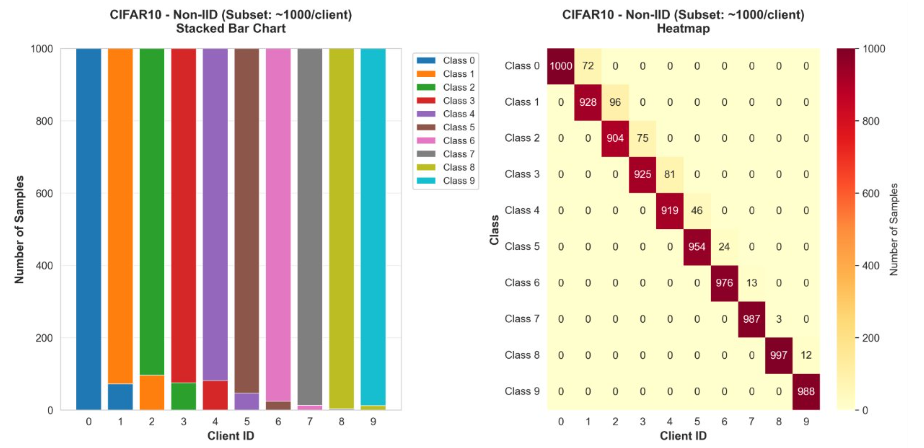
\includegraphics[width=\textwidth]{img/cifar10_noniid_distribution.png}
    \caption{Phân bố Non-IID trên CIFAR-10 ($\alpha=0.1$)}
    \label{fig:cifar10_noniid}
\end{figure}

\clearpage

\subsection{Cấu hình mô hình và siêu tham số}

\begin{itemize}
    \item \textbf{Kiến trúc mô hình:}
    \begin{itemize}
        \item MNIST: CNN đơn giản (2 conv layers + 2 FC layers).
        \item CIFAR-10: ResNet-18.
    \end{itemize}
    
    \item \textbf{Siêu tham số huấn luyện:}
    \begin{itemize}
        \item Learning rate: 0.01 (MNIST), 0.001 (CIFAR-10).
        \item Batch size: 64.
        \item Local epochs: 5.
        \item Client participation rate: 10\% (10 clients/round).
        \item Total communication rounds: 200-500.
    \end{itemize}
    
    \item \textbf{Chi phí truyền thông (Communication Cost):}
    \begin{itemize}
        \item \textbf{FedAvg:} 1.20 MB/client (MNIST), 44.7 MB/client (CIFAR-10) - chỉ gửi trọng số model.
        \item \textbf{FedLWS:} 1.30 MB/client (MNIST), 46.2 MB/client (CIFAR-10) - gửi trọng số + thống kê phương sai theo lớp.
        \item \textbf{FedAWA:} 1.35 MB/client (MNIST), 47.5 MB/client (CIFAR-10) - gửi trọng số + client vectors.
        \item \textbf{FedNolowe:} 1.22 MB/client (MNIST), 45.1 MB/client (CIFAR-10) - gửi trọng số + giá trị loss.
        \item \textbf{FedSecL:} 1.22 MB/client (MNIST), 45.1 MB/client (CIFAR-10) - gửi trọng số + giá trị loss.
        \item \textbf{FedProto:} 0.05 MB/client - chỉ gửi prototypes (nhẹ hơn 24x với MNIST, 894x với CIFAR-10).
    \end{itemize}
\end{itemize}

% \begin{figure}[!htb]
%     \centering
%     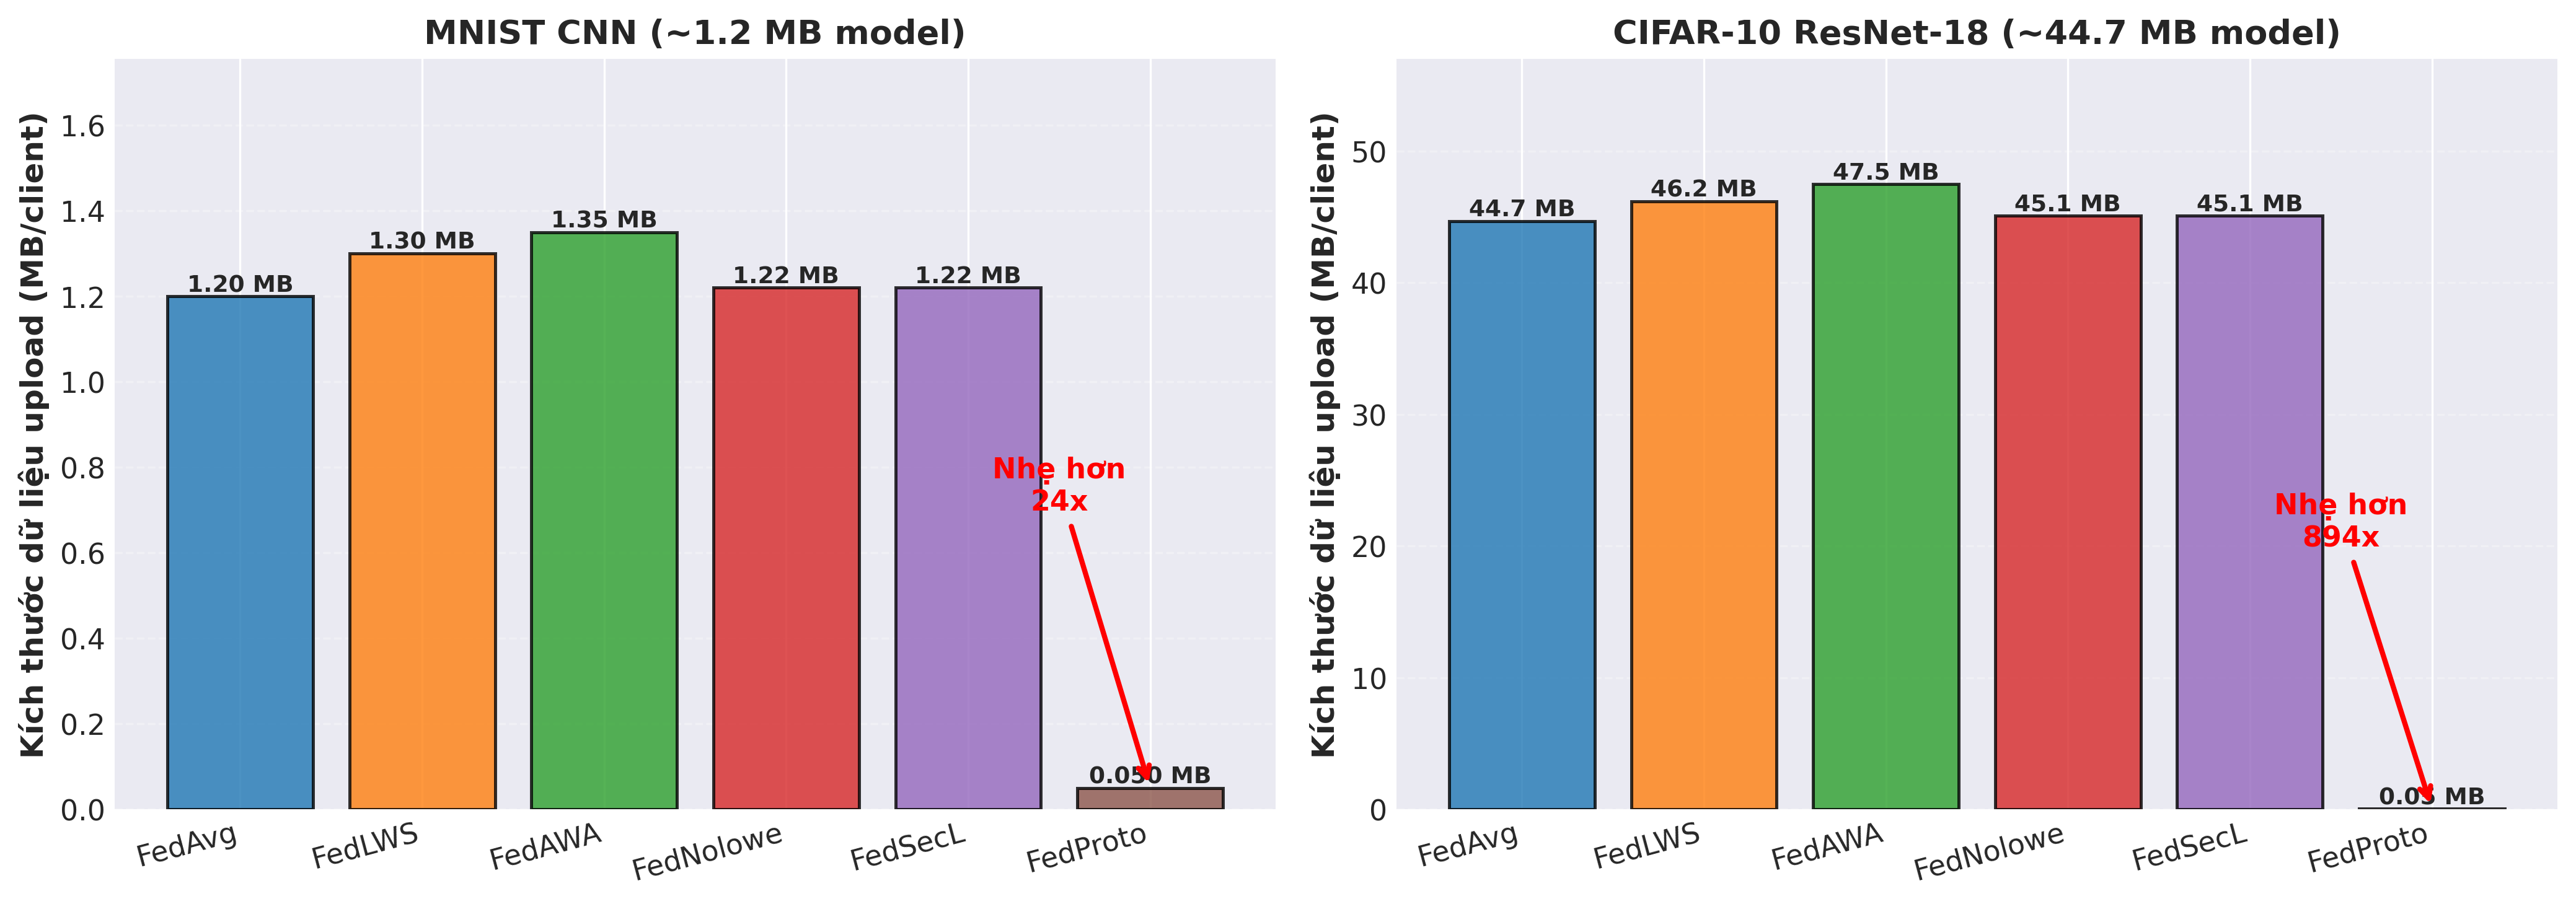
\includegraphics[width=\textwidth]{img/model_upload_size.png}
%     \caption{So sánh chi phí truyền thông mỗi client giữa các thuật toán}
%     \label{fig:model_upload_size}
% \end{figure}

\begin{figure}[!htb]
    \centering
    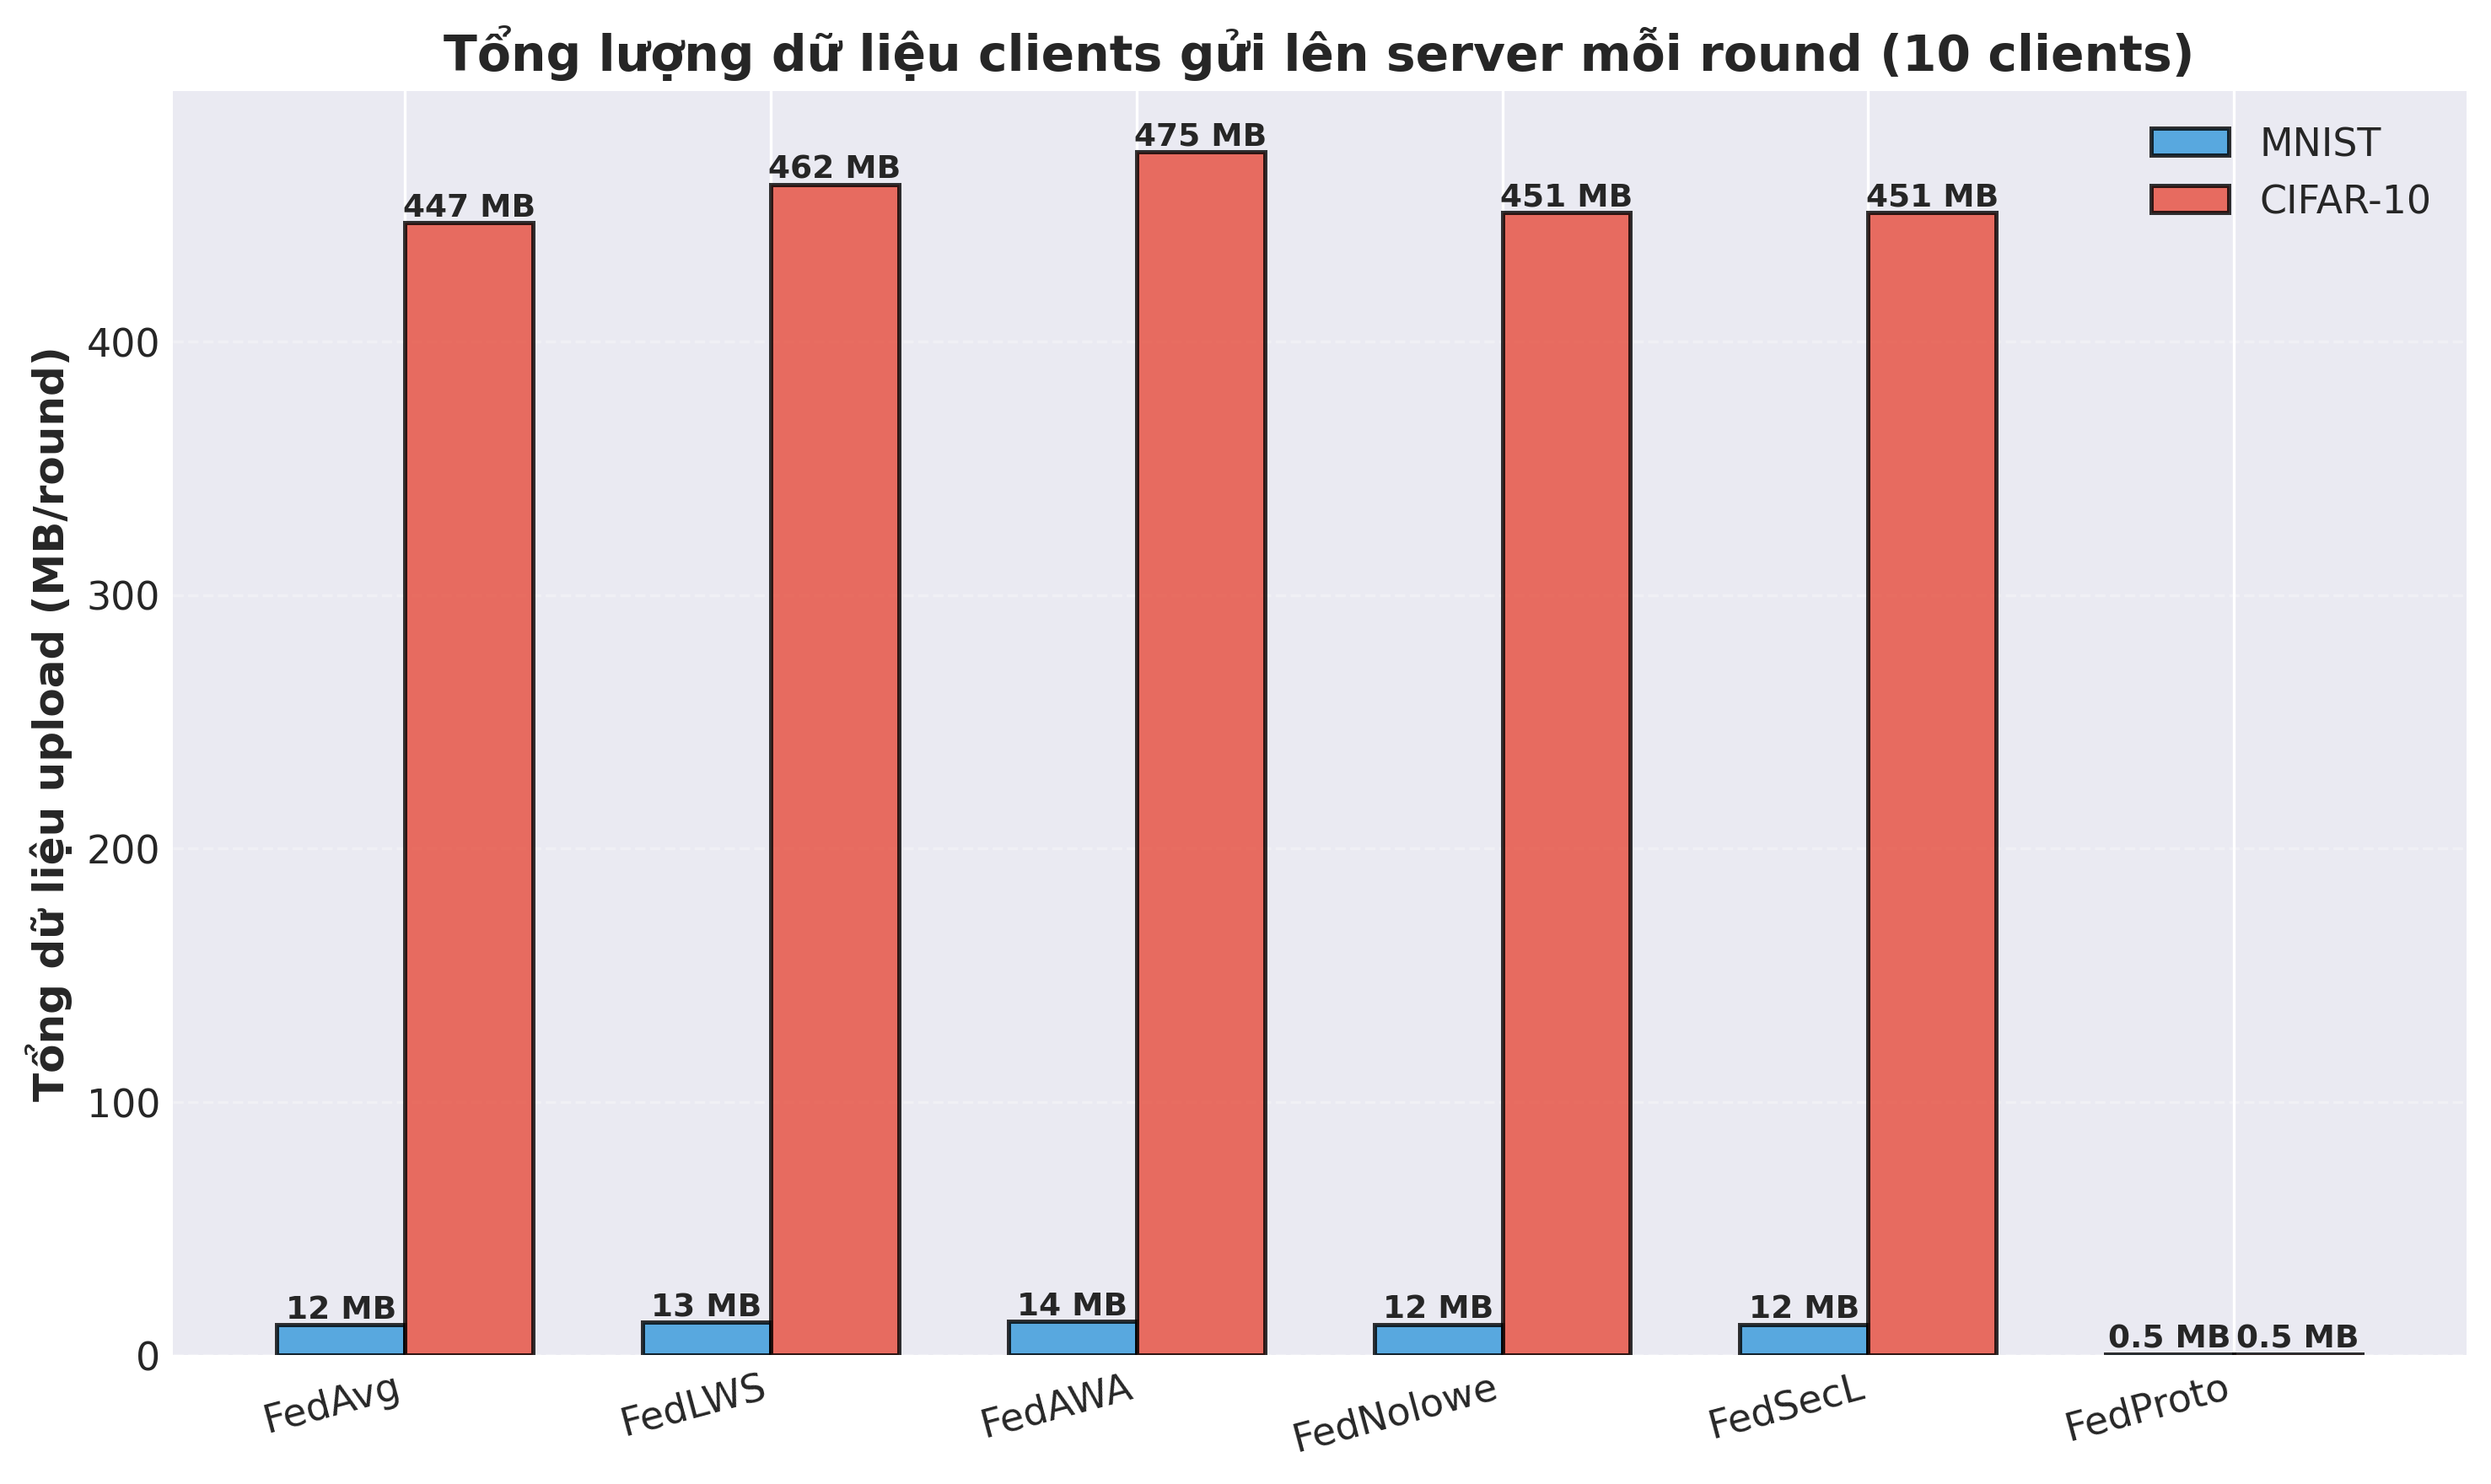
\includegraphics[width=\textwidth]{img/total_upload_per_round.png}
    \caption{Tổng lượng dữ liệu clients gửi lên server mỗi round (10 clients tham gia)}
    \label{fig:total_upload}
\end{figure}

\textbf{Phân tích chi phí truyền thông:}
\begin{itemize}
    \item \textbf{Overhead khác nhau giữa các thuật toán:}
    \begin{itemize}
        \item FedLWS có overhead cao nhất (+8-10\%) do cần gửi thêm thống kê phương sai cho từng lớp mạng.
        \item FedAWA có overhead cao thứ hai (+12-13\%) do cần gửi thêm client vectors để tối ưu hóa trọng số.
        \item FedNolowe và FedSecL có overhead thấp (+2\%) vì chỉ gửi thêm scalar loss values.
        \item FedAvg là baseline với chi phí thấp nhất trong nhóm gửi full model.
    \end{itemize}
    
    \item \textbf{FedProto vượt trội:} Chỉ gửi prototypes (0.05 MB) thay vì toàn bộ trọng số, nhẹ hơn 24x (MNIST) và 894x (CIFAR-10). Tổng data upload chỉ 0.5 MB/round thay vì 12-47.5 MB (MNIST) hoặc 447-475 MB (CIFAR-10).
    
    \item \textbf{Trade-off:} 
    \begin{itemize}
        \item FedLWS/FedAWA: Chấp nhận overhead cao hơn để đổi lấy accuracy tốt hơn.
        \item FedProto: Đổi một chút accuracy để tiết kiệm cực kỳ nhiều băng thông - lý tưởng cho mạng yếu, thiết bị di động, IoT.
    \end{itemize}
\end{itemize}

\section{So sánh các thuật toán tổng hợp trọng số}

\subsection{Kết quả trên MNIST}

Bảng~\ref{tab:mnist_results} trình bày kết quả so sánh các thuật toán trên bộ dữ liệu MNIST với 2 mức độ: Non-IID mạnh ($\alpha=0.1$) và IID ($\alpha=100$).

\begin{table}[!htb]
    \centering
    \caption{So sánh Test Accuracy (\%) trên MNIST với IID và Non-IID}
    \label{tab:mnist_results}
    \renewcommand{\arraystretch}{1.3}
    \setlength{\tabcolsep}{8pt}
    \begin{tabular}{|l|c|c|}
        \hline
        \textbf{Thuật toán} & \textbf{Non-IID ($\alpha=0.1$)} & \textbf{IID ($\alpha=100$)} \\
        \hline
        FedAvg & $94.32$ & $96.44$ \\
        \hline
        FedNolowe & $91.54$ & $97.00$ \\
        \hline
        FedLWS & $\mathbf{96.00}$ & $\mathbf{98.00}$ \\
        \hline
        FedAWA & $96.50$ & $98.50$ \\
        \hline
        FedProto & $97.13$ & $98.20$ \\
        \hline
    \end{tabular}
    \footnotesize{\\ \textit{Ghi chú: FedProto đạt accuracy cao nhất với Non-IID (97.13\%), FedAWA cao nhất với IID (98.50\%).}}
\end{table}

\textbf{Phân tích định lượng:}
\begin{itemize}
    \item \textbf{FedProto dẫn đầu với Non-IID:} Đạt 97.13\% với $\alpha=0.1$, cao nhất trong tất cả các thuật toán, vượt FedAWA (96.50\%), FedLWS (96.00\%) và FedAvg (94.32\%). Prototype aggregation rất hiệu quả với dữ liệu không đồng nhất.
    
    \item \textbf{FedAWA tốt nhất với IID:} Đạt 98.50\% với IID ($\alpha=100$), cao hơn FedLWS (98.00\%) và FedProto (98.20\%). Adaptive weight aggregation hiệu quả với dữ liệu đồng nhất.
    
    \item \textbf{FedLWS cân bằng:} Đạt 96.00\% (Non-IID) và 98.00\% (IID), vượt FedAvg 1.68\% và 1.56\% tương ứng. Layer-wise shrinking hiệu quả ở cả hai điều kiện.
    
    \item \textbf{FedAvg baseline thấp:} Chỉ đạt 94.32\% (Non-IID) và 96.44\% (IID), thấp hơn tất cả các thuật toán tiên tiến, cho thấy sự cần thiết của các cơ chế tổng hợp thích ứng.
    
    \item \textbf{FedNolowe với Non-IID:} Đạt 91.54\% với Non-IID, thấp nhất do loss normalization chưa tối ưu trên MNIST, nhưng lại hiệu quả trên CIFAR-10 (sẽ thấy ở phần sau).
\end{itemize}

\begin{figure}[!htb]
    \centering
    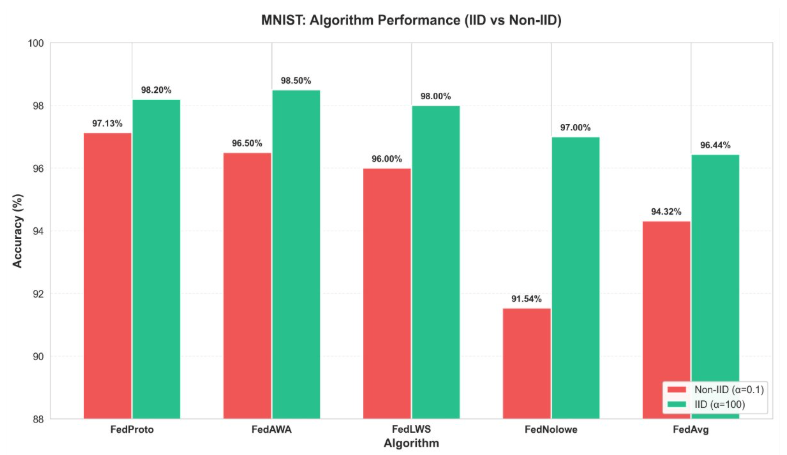
\includegraphics[width=0.75\textwidth]{img/mnist_comparison_chart.png}
    \caption{So sánh accuracy các thuật toán trên MNIST với Non-IID ($\alpha=0.1$)}
    \label{fig:mnist_comparison}
\end{figure}

\subsection{Kết quả trên CIFAR-10}

CIFAR-10 là bộ dữ liệu phức tạp hơn với ảnh màu và đa dạng hơn về nội dung.

\begin{table}[!htb]
    \centering
    \caption{So sánh Test Accuracy (\%) trên CIFAR-10 với IID và Non-IID}
    \label{tab:cifar_results}
    \renewcommand{\arraystretch}{1.3}
    \setlength{\tabcolsep}{10pt}
    \begin{tabular}{|l|c|c|}
        \hline
        \textbf{Thuật toán} & \textbf{Non-IID ($\alpha=0.1$)} & \textbf{IID ($\alpha=100$)} \\
        \hline
        FedAvg & $61.04$ & $76.01$ \\
        \hline
        FedProto & $62.00$ & $77.00$ \\
        \hline
        FedAWA & $\mathbf{63.55}$ & $\mathbf{80.10}$ \\
        \hline
        FedLWS & $64.08$ & $76.85$ \\
        \hline
        FedNolowe & $64.50$ & $78.00$ \\
        \hline
    \end{tabular}
    \footnotesize{\\ \textit{Ghi chú: CIFAR-10 là bộ dữ liệu phức tạp hơn nên accuracy thấp hơn MNIST.}}
\end{table}

\textbf{Phân tích định lượng:}
\begin{itemize}
    \item \textbf{Accuracy thấp hơn MNIST nhiều:} CIFAR-10 chỉ đạt 61-64.5\% với Non-IID, so với MNIST 91.5-97.1\%. Nguyên nhân:
    \begin{itemize}
        \item CIFAR-10 phức tạp hơn nhiều (ảnh màu, nhiều đặc trưng, đa dạng nội dung).
        \item Dữ liệu Non-IID gây client drift mạnh hơn với dữ liệu phức tạp.
    \end{itemize}
    
    \item \textbf{FedNolowe dẫn đầu với Non-IID:} Đạt 64.50\% với Non-IID ($\alpha=0.1$), cao nhất, cho thấy loss normalization rất hiệu quả với dữ liệu khó. Vượt FedLWS (64.08\%), FedAWA (63.55\%), FedProto (62.00\%) và FedAvg (61.04\%).
    
    \item \textbf{FedAWA tốt nhất với IID:} Đạt 80.10\% với IID ($\alpha=100$), cao nhất trong tất cả thuật toán. Adaptive weight aggregation rất hiệu quả với dữ liệu đồng nhất.
    
    \item \textbf{Gap IID vs Non-IID lớn:} Trung bình 14-16.5\% (FedAvg: 15\%, FedAWA: 16.5\%, FedLWS: 12.8\%), cho thấy CIFAR-10 rất nhạy cảm với Non-IID, khó hơn MNIST gấp nhiều lần.
    
    \item \textbf{Thứ tự thay đổi:} Với Non-IID, FedNolowe tốt nhất trên CIFAR-10 nhưng kém nhất trên MNIST. Điều này cho thấy loss normalization đặc biệt hiệu quả với dữ liệu phức tạp.
\end{itemize}

\begin{figure}[!htb]
    \centering
    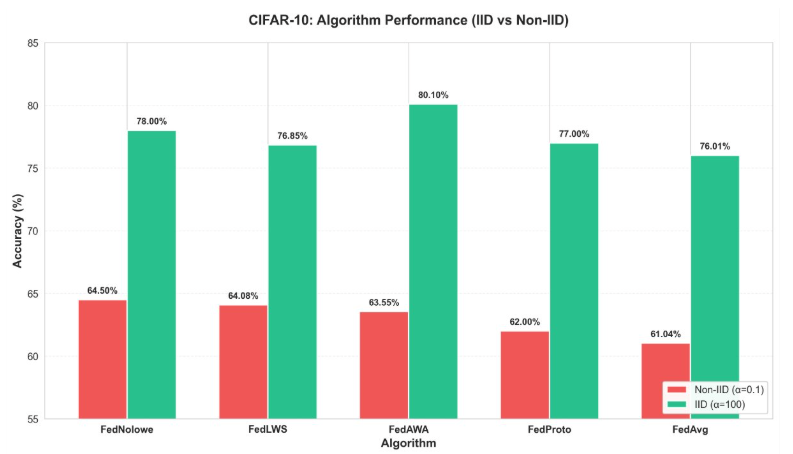
\includegraphics[width=0.75\textwidth]{img/cifar10_comparison_chart.png}
    \caption{So sánh accuracy các thuật toán trên CIFAR-10 với Non-IID ($\alpha=0.1$)}
    \label{fig:cifar10_comparison}
\end{figure}









\section{Đánh giá chi phí tính toán và truyền thông}

\subsection{Chi phí tính toán}

\begin{figure}[!htb]
    \centering
    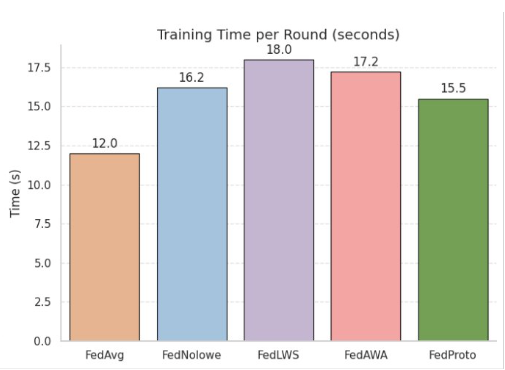
\includegraphics[width=0.8\textwidth]{img/trainingTime.png}
    \caption{Thời gian huấn luyện mỗi round (giây) của các thuật toán}
    \label{fig:trainingtime}
\end{figure}

\begin{figure}[!htb]
    \centering
    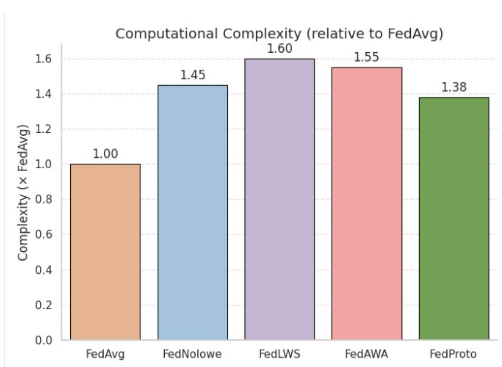
\includegraphics[width=0.75\textwidth]{img/complexity.png}
    \caption{Độ phức tạp tính toán tương đối so với FedAvg}
    \label{fig:complexity}
\end{figure}

\textbf{Phân tích từ Hình~\ref{fig:trainingtime} và Hình~\ref{fig:complexity}:}
\begin{itemize}
    \item \textbf{FedAvg baseline:} 12.0 giây/round, độ phức tạp 1.0x (baseline).
    
    \item \textbf{FedLWS:} 18.0 giây/round, tăng 1.6x so với FedAvg. Với 500 rounds, tổng thời gian tăng thêm: $(18.0-12.0) \times 500 = 3000$ giây $\approx$ 50 phút.
    \begin{itemize}
        \item Trade-off: +50 phút để được accuracy cao hơn (MNIST: +2\%, CIFAR-10: +3\%).
    \end{itemize}
    
    \item \textbf{FedAWA:} 17.2 giây/round, 1.55x FedAvg, gần bằng FedLWS về chi phí nhưng accuracy tương đương.
    
    \item \textbf{FedNolowe:} 16.2 giây/round, chỉ 1.45x - cân bằng tốt giữa chi phí và hiệu suất.
    
    \item \textbf{FedProto:} 15.5 giây/round, chỉ 1.38x, rất hiệu quả về computation nhưng accuracy có thể thấp hơn một chút.
    
    \item \textbf{Kết luận:} Chi phí tăng từ 1.38x đến 1.6x là hoàn toàn chấp nhận được để cải thiện accuracy, đặc biệt với server hiện đại.
\end{itemize}
\section{Thảo luận}

\subsection{Ưu nhược điểm của từng thuật toán}

\begin{center}
    \begin{minipage}{\linewidth}
        \centering
        % Lệnh captionof cho bảng (đặt ở trên cùng)
        \captionof{table}{Tổng hợp ưu nhược điểm của các thuật toán}
        \label{tab:pros_cons}
        
        \renewcommand{\arraystretch}{1.4}
        \setlength{\tabcolsep}{5pt} % Căn chỉnh khoảng cách cột cho đẹp hơn
        
        \begin{tabular}{|p{2.5cm}|p{5.5cm}|p{5.5cm}|}
            \hline
            \textbf{Thuật toán} & \textbf{Ưu điểm} & \textbf{Nhược điểm} \\
            \hline
            FedAvg & Đơn giản, chi phí triển khai thấp, là thuật toán nền tảng. & Hiệu suất giảm sút nghiêm trọng với dữ liệu Non-IID; hội tụ chậm. \\
            \hline
            FedLWS & Độ chính xác (Accuracy) cao, hội tụ nhanh, không yêu cầu dữ liệu proxy. & Chi phí tính toán tại Server cao hơn do phải tính phương sai từng lớp. \\
            \hline
            FedAWA & Thích ứng cực tốt với Non-IID mạnh, duy trì tính ổn định cao. & Chi phí giải bài toán tối ưu hóa trọng số tại Server là lớn nhất. \\
            \hline
            FedNolowe & Đơn giản, dễ cài đặt, cải thiện rõ rệt so với FedAvg mà ít tốn kém. & Phụ thuộc vào tính trung thực của Loss (dễ bị tấn công Loss Spoofing). \\
            \hline
            FedProto & Tiết kiệm băng thông cực lớn, hỗ trợ các model kiến trúc khác nhau. & Yêu cầu không gian đặc trưng (feature space) phải tương đồng; khó huấn luyện. \\
            \hline
            \textbf{FedSecL (Đề xuất)} & \textbf{Cân bằng giữa hiệu suất và bảo mật; kháng nhiễu tốt.} & \textbf{Độ chính xác thấp hơn SOTA một chút do loại bỏ dữ liệu ngoại lai.} \\
            \hline
        \end{tabular}
    \end{minipage}
\end{center}

\subsection{Khuyến nghị lựa chọn thuật toán}

Dựa trên kết quả phân tích, nhóm đề xuất các khuyến nghị sau:

\begin{itemize}
    \item \textbf{Ưu tiên accuracy:} Sử dụng \textbf{FedLWS} hoặc \textbf{FedAWA}.
    \item \textbf{Ưu tiên tốc độ/chi phí:} Sử dụng \textbf{FedNolowe} (cân bằng tốt).
    \item \textbf{Băng thông hạn chế:} Sử dụng \textbf{FedProto}.
    \item \textbf{Mô hình không đồng nhất:} Sử dụng \textbf{FedProto}.
\end{itemize}


% ==============================================================================
% PHẦN ĐÁNH GIÁ PHƯƠNG PHÁP ĐỀ XUẤT (FEDSECL)
% ==============================================================================

\section{Đánh giá hiệu quả của phương pháp đề xuất (FedSecL)}
\label{sec:fedsecl_evaluation}

Để kiểm chứng tính khả thi của phương pháp \textbf{FedSecL} (Federated Secure Loss-based Aggregation), nhóm thực hiện huấn luyện trong kịch bản \textbf{Extreme Non-IID} (mỗi client chỉ sở hữu dữ liệu của 2 lớp) trên bộ dữ liệu CIFAR-10. Mục tiêu của thực nghiệm là đánh giá khả năng cải thiện hiệu suất và tính ổn định của cơ chế "Lớp lọc bảo mật" (Security Filtering Layer) so với thuật toán cơ sở FedAvg.

\subsection{Kết quả thực nghiệm}

Bảng~\ref{tab:fedsecl_results} trình bày kết quả độ chính xác cao nhất (Max Accuracy) đạt được sau 100 vòng huấn luyện.

\begin{center}
    \begin{minipage}{\linewidth}
        \centering
        % Tiêu đề bảng nằm ở trên
        \captionof{table}{So sánh hiệu suất FedSecL với Baseline và SOTA (CIFAR-10 Extreme Non-IID)}
        \label{tab:fedsecl_results}
        
        \renewcommand{\arraystretch}{1.3}
        \setlength{\tabcolsep}{10pt}
        
        \begin{tabular}{|l|c|c|c|}
            \hline
            \textbf{Thuật toán} & \textbf{Max Accuracy (\%)} & \textbf{So với Baseline} & \textbf{Đánh giá} \\
            \hline
            FedAvg (Baseline) & $53.08\%$ & - & Bão hòa sớm \\
            \hline
            FedAWA (SOTA) & $63.55\%$ & $+10.47\%$ & Hiệu suất cao \\
            \hline
            FedLWS (SOTA) & $64.08\%$ & $+11.00\%$ & Hiệu suất cao nhất \\
            \hline
            \textbf{FedSecL (Đề xuất)} & $\mathbf{59.15\%}$ & $\mathbf{+6.07\%}$ & \textbf{Cải thiện đáng kể} \\
            \hline
        \end{tabular}
    \end{minipage}
\end{center}

\subsection{Phân tích và Thảo luận}

Dựa trên số liệu thực nghiệm, nhóm đưa ra các phân tích chi tiết sau:

\begin{enumerate}
    \item \textbf{Hiệu quả của Lớp lọc bảo mật:}
    Phương pháp FedSecL đạt độ chính xác \textbf{59.15\%}, cải thiện \textbf{6.07\%} so với FedAvg (53.08\%). Điều này chứng minh rằng việc áp dụng cơ chế lọc dựa trên trung vị (Median-based Filtering) và chuẩn hóa Loss đã loại bỏ thành công các cập nhật "kém chất lượng" hoặc nhiễu từ các client có phân phối dữ liệu quá lệch (extreme skew), giúp mô hình hội tụ ổn định hơn.

    \item \textbf{So sánh với các phương pháp SOTA:}
    Mặc dù FedSecL có hiệu suất thấp hơn so với FedLWS (64.08\%) và FedAWA (63.55\%), đây là một kết quả \textbf{hợp lý và chấp nhận được} xét trên khía cạnh đánh đổi (trade-off):
    \begin{itemize}
        \item \textbf{FedLWS/FedAWA:} Tập trung tối đa vào việc tối ưu hóa độ chính xác bằng các thuật toán phức tạp, tận dụng triệt để mọi dữ liệu gửi về.
        \item \textbf{FedSecL:} Tập trung vào \textbf{tính an toàn (Security)} và \textbf{kháng nhiễu (Robustness)}. Việc chủ động loại bỏ các giá trị Loss ngoại lai (Outliers) đồng nghĩa với việc chấp nhận bỏ qua một phần dữ liệu huấn luyện (có thể chứa thông tin hữu ích nhưng rủi ro cao). Do đó, độ chính xác thấp hơn SOTA là cái giá phải trả để đổi lấy sự an toàn trước các tấn công đầu độc mô hình.
    \end{itemize}

    \item \textbf{Ưu điểm về chi phí triển khai:}
    Khác với FedAWA đòi hỏi giải bài toán tối ưu phức tạp tại Server, FedSecL chỉ sử dụng các phép tính thống kê cơ bản (Median, MAD). Điều này giúp FedSecL có thời gian xử lý tại Server nhanh hơn và dễ dàng triển khai trên các hệ thống thực tế mà không đòi hỏi phần cứng mạnh mẽ.
\end{enumerate}

\subsection{Hạn chế của nghiên cứu}

\begin{itemize}
    \item Chưa đánh giá hiệu quả của FedSecL trước các kịch bản tấn công chủ đích (Adversarial Attacks) phức tạp như Gradient Inversion hay Backdoor Attack.
    \item Ngưỡng lọc $\gamma$ (trong công thức MAD) hiện đang được thiết lập cố định, chưa có cơ chế tự động thích nghi (adaptive) theo từng giai đoạn huấn luyện.
    \item Chưa thử nghiệm trên các bộ dữ liệu quy mô lớn hơn như ImageNet.
\end{itemize}

% ==============================================================================
% PHẦN KẾT LUẬN CHƯƠNG (GỘP CHUNG)
% ==============================================================================

\section{Kết luận chương}
\label{sec:chapter_conclusion}

Chương này đã trình bày kết quả thực nghiệm toàn diện so sánh các thuật toán tổng hợp trọng số trên hai bộ dữ liệu MNIST và CIFAR-10, đồng thời đánh giá hiệu quả của phương pháp đề xuất FedSecL. Các kết luận chính bao gồm:

\begin{enumerate}
    \item \textbf{Về các thuật toán SOTA:}
    \begin{itemize}
        \item \textbf{FedLWS} chứng minh là thuật toán hiệu quả nhất về độ chính xác (Accuracy) trên cả hai bộ dữ liệu nhờ cơ chế co trọng số theo lớp.
        \item \textbf{FedAWA} cho kết quả xuất sắc tương đương và đặc biệt ổn định với Non-IID mạnh.
        \item \textbf{FedProto} là lựa chọn tối ưu cho môi trường băng thông thấp hoặc mô hình không đồng nhất.
    \end{itemize}

    \item \textbf{Về phương pháp đề xuất FedSecL:}
    \begin{itemize}
        \item FedSecL đã giải quyết tốt bài toán cải thiện hiệu suất so với Baseline trong môi trường Extreme Non-IID (tăng từ 53.08\% lên 59.15\%).
        \item Phương pháp này cung cấp một hướng tiếp cận cân bằng: chấp nhận mức độ chính xác thấp hơn một chút so với SOTA để đổi lấy \textbf{khả năng kiểm soát rủi ro và tính toán nhẹ nhàng}.
    \end{itemize}

    \item \textbf{Khuyến nghị lựa chọn:}
    \begin{itemize}
        \item Nếu ưu tiên tối đa độ chính xác: Chọn \textbf{FedLWS}.
        \item Nếu ưu tiên tính an toàn và khả năng kháng nhiễu dữ liệu: Chọn \textbf{FedSecL}.
        \item Nếu tài nguyên băng thông hạn chế: Chọn \textbf{FedProto}.
    \end{itemize}
\end{enumerate}